%! Author: Facundo Bautista Barbera
%! Date: 2025-10-16
%! TEX root = tarea_4_mr.tex

\documentclass{article}

\usepackage{amsmath}
\usepackage{amssymb}
\usepackage[spanish]{babel}
\usepackage{graphicx}

\title{Tarea 4 MR: Simulación de Taller}
\author{Facundo Bautista Barbera}
\date{\today}

\begin{document}
\maketitle

\section*{Planteamiento del problema}

Suponga que el tiempo necesario para fabricar una parte en una máquina se describe con la siguiente distribución uniforme:

$$f(t) = \frac{1}{b-a}, \quad a \leq t \leq b$$

En un taller con una sola máquina se reciben trabajos en forma aleatoria. El tiempo entre llegadas tiene una distribución exponencial, con una media de 2 horas. El tiempo necesario para procesar un trabajo tiene una distribución uniforme entre 1.1 y 2 horas. Suponiendo que el primer trabajo llegue cuando el tiempo es 0.

\section*{Parte a) Ecuación para el tiempo $t$ dado el número aleatorio $R$}

Para generar variables aleatorias a partir de números uniformes $R \sim U(0,1)$, utilizamos el método de la transformada inversa.

\textbf{Distribución Uniforme $U(a,b)$}

\vspace{0.3cm}
La función de distribución acumulada es:
$$F(t) = \frac{t-a}{b-a}, \quad a \leq t \leq b$$

Igualando $F(t) = R$ y despejando $t$:
$$R = \frac{t-a}{b-a}$$
$$t = a + (b-a)R$$

Para nuestro caso con $a = 1.1$ y $b = 2$:
$$\boxed{t_2 = 1.1 + 0.9R}$$

donde $t_2$ es el tiempo de procesamiento.

\vspace{0.5cm}
\textbf{Distribución Exponencial con media $\mu = 2$}

\vspace{0.3cm}
La función de distribución acumulada es:
$$F(t) = 1 - e^{-t/\mu} = 1 - e^{-t/2}$$

Igualando $F(t) = R$ y despejando $t$:
$$R = 1 - e^{-t/2}$$
$$e^{-t/2} = 1 - R$$
$$-\frac{t}{2} = \ln(1-R)$$
$$\boxed{t_1 = -2\ln(1-R)}$$

donde $t_1$ es el tiempo entre llegadas.

\textit{Nota:} Como $R \sim U(0,1)$, entonces $(1-R) \sim U(0,1)$, por lo que también se puede usar $t_1 = -2\ln(R)$.

\newpage

\section*{Parte b) Simulación de los primeros 5 trabajos}

Usando los primeros cinco números aleatorios de la primera columna de la TABLA 18.1 para generar tiempos entre llegadas, y los de la segunda columna para tiempos de procesamiento:

\textbf{Columna 1 (para $t_1$):} 0.0589, 0.6733, 0.4799, 0.9486, 0.6139

\textbf{Columna 2 (para $t_2$):} 0.3529, 0.3646, 0.7676, 0.8931, 0.3919

\vspace{0.5cm}
\textbf{Cálculos detallados:}

\vspace{0.3cm}
\textbf{Cliente 1:}
\begin{itemize}
    \item Hora de llegada: 0 (dado en el problema)
    \item Tiempo de procesamiento: $t_2 = 1.1 + 0.9(0.3529) = 1.4176$
    \item Hora de inicio: 0 (máquina libre)
    \item Hora de salida: $0 + 1.4176 = 1.4176$
\end{itemize}

\textbf{Cliente 2:}
\begin{itemize}
    \item Tiempo entre llegadas: $t_1 = -2\ln(0.0589) = 5.6632$
    \item Hora de llegada: $0 + 5.6632 = 5.6632$
    \item Tiempo de procesamiento: $t_2 = 1.1 + 0.9(0.3646) = 1.4281$
    \item Hora de inicio: 5.6632 (máquina libre desde 1.4176)
    \item Hora de salida: $5.6632 + 1.4281 = 7.0913$
\end{itemize}

\textbf{Cliente 3:}
\begin{itemize}
    \item Tiempo entre llegadas: $t_1 = -2\ln(0.6733) = 0.7913$
    \item Hora de llegada: $5.6632 + 0.7913 = 6.4545$
    \item Tiempo de procesamiento: $t_2 = 1.1 + 0.9(0.7676) = 1.7908$
    \item Hora de inicio: 7.0913 (máquina ocupada hasta entonces)
    \item Hora de salida: $7.0913 + 1.7908 = 8.8821$
\end{itemize}

\textbf{Cliente 4:}
\begin{itemize}
    \item Tiempo entre llegadas: $t_1 = -2\ln(0.4799) = 1.4676$
    \item Hora de llegada: $6.4545 + 1.4676 = 7.9221$
    \item Tiempo de procesamiento: $t_2 = 1.1 + 0.9(0.8931) = 1.9038$
    \item Hora de inicio: 8.8821 (máquina ocupada)
    \item Hora de salida: $8.8821 + 1.9038 = 10.7859$
\end{itemize}

\textbf{Cliente 5:}
\begin{itemize}
    \item Tiempo entre llegadas: $t_1 = -2\ln(0.9486) = 0.1057$
    \item Hora de llegada: $7.9221 + 0.1057 = 8.0278$
    \item Tiempo de procesamiento: $t_2 = 1.1 + 0.9(0.3919) = 1.4527$
    \item Hora de inicio: 10.7859 (máquina ocupada)
    \item Hora de salida: $10.7859 + 1.4527 = 12.2386$
\end{itemize}

\vspace{0.5cm}
\textbf{Tabla resumen:}

\vspace{0.3cm}
\begin{center}
\begin{tabular}{|c|c|c|c|c|c|c|}
\hline
\textbf{Cliente} & \textbf{R (t1)} & \textbf{t1} & \textbf{Hora llegada} & \textbf{R (t2)} & \textbf{t2} & \textbf{Hora salida} \\
\hline
1 & - & - & 0.0000 & 0.3529 & 1.4176 & 1.4176 \\
2 & 0.0589 & 5.6632 & 5.6632 & 0.3646 & 1.4281 & 7.0913 \\
3 & 0.6733 & 0.7913 & 6.4545 & 0.7676 & 1.7908 & 8.8821 \\
4 & 0.4799 & 1.4676 & 7.9221 & 0.8931 & 1.9038 & 10.7859 \\
5 & 0.9486 & 0.1057 & 8.0278 & 0.3919 & 1.4527 & 12.2386 \\
\hline
\end{tabular}
\end{center}

\newpage

\section*{Parte c) Simulación completa con 60 trabajos}

Para realizar la simulación completa con 60 trabajos, se utilizan los números aleatorios de la TABLA 18.1. Se implementó un programa en Python que:

\begin{enumerate}
    \item Lee los números aleatorios de la tabla (columna 1 para llegadas, columna 2 para procesamientos)
    \item Genera tiempos entre llegadas usando distribución exponencial ($\mu = 2$)
    \item Genera tiempos de procesamiento usando distribución uniforme $[1.1, 2]$
    \item Simula el sistema de colas considerando si la máquina está libre u ocupada
    \item Calcula estadísticas del sistema
\end{enumerate}

\vspace{0.3cm}
El código completo se encuentra en el archivo \texttt{simulacion.py} adjunto.

\vspace{0.5cm}
\textbf{Estadísticas del sistema:}
\begin{itemize}
    \item Tiempo total de simulación: 105.4364 horas
    \item Utilización de la máquina: 95.15\%
    \item Tiempo promedio en el sistema: 4.4098 horas
    \item Tiempo promedio de espera: 2.7377 horas
    \item Tiempo promedio de servicio: 1.6720 horas
    \item Número de clientes atendidos: 60
\end{itemize}

\vspace{0.5cm}
\textbf{Tabla de primeros 10 trabajos:}

\vspace{0.3cm}
\begin{center}
\small
\begin{tabular}{|c|c|c|c|c|c|c|}
\hline
\textbf{Cliente} & \textbf{R (t1)} & \textbf{t1} & \textbf{Llegada} & \textbf{R (t2)} & \textbf{t2} & \textbf{Salida} \\
\hline
1 & - & - & 0.0000 & 0.3529 & 1.4176 & 1.4176 \\
2 & 0.0589 & 5.6638 & 5.6638 & 0.3646 & 1.4281 & 7.0920 \\
3 & 0.6733 & 0.7911 & 6.4550 & 0.7676 & 1.7908 & 8.8828 \\
4 & 0.4799 & 1.4684 & 7.9233 & 0.8931 & 1.9038 & 10.7866 \\
5 & 0.9486 & 0.1055 & 8.0288 & 0.3919 & 1.4527 & 12.2393 \\
6 & 0.6139 & 0.9758 & 9.0047 & 0.7876 & 1.8088 & 14.0481 \\
7 & 0.5933 & 1.0441 & 10.0488 & 0.5199 & 1.5679 & 15.6161 \\
8 & 0.9341 & 0.1363 & 10.1851 & 0.6358 & 1.6722 & 17.2883 \\
9 & 0.1782 & 3.4497 & 13.6348 & 0.7472 & 1.7725 & 19.0608 \\
10 & 0.3473 & 2.1151 & 15.7500 & 0.8954 & 1.9059 & 20.9666 \\
\hline
\end{tabular}
\end{center}

\newpage

\textbf{Análisis de resultados:}

\begin{itemize}
    \item La utilización de la máquina es del 95.15\%, lo que indica que el sistema está altamente ocupado.
    \item El tiempo promedio de espera (2.74 horas) representa aproximadamente el 62\% del tiempo total en el sistema.
    \item El sistema está cercano a la saturación, ya que $\lambda \approx 0.57$ trabajos/hora y $\mu_{\text{servicio}} \approx 0.60$ trabajos/hora.
    \item Los resultados completos se encuentran en \texttt{resultados\_simulacion.csv}.
\end{itemize}

\vspace{0.5cm}
\textbf{Gráficas de la simulación:}

\begin{figure}[h]
\centering
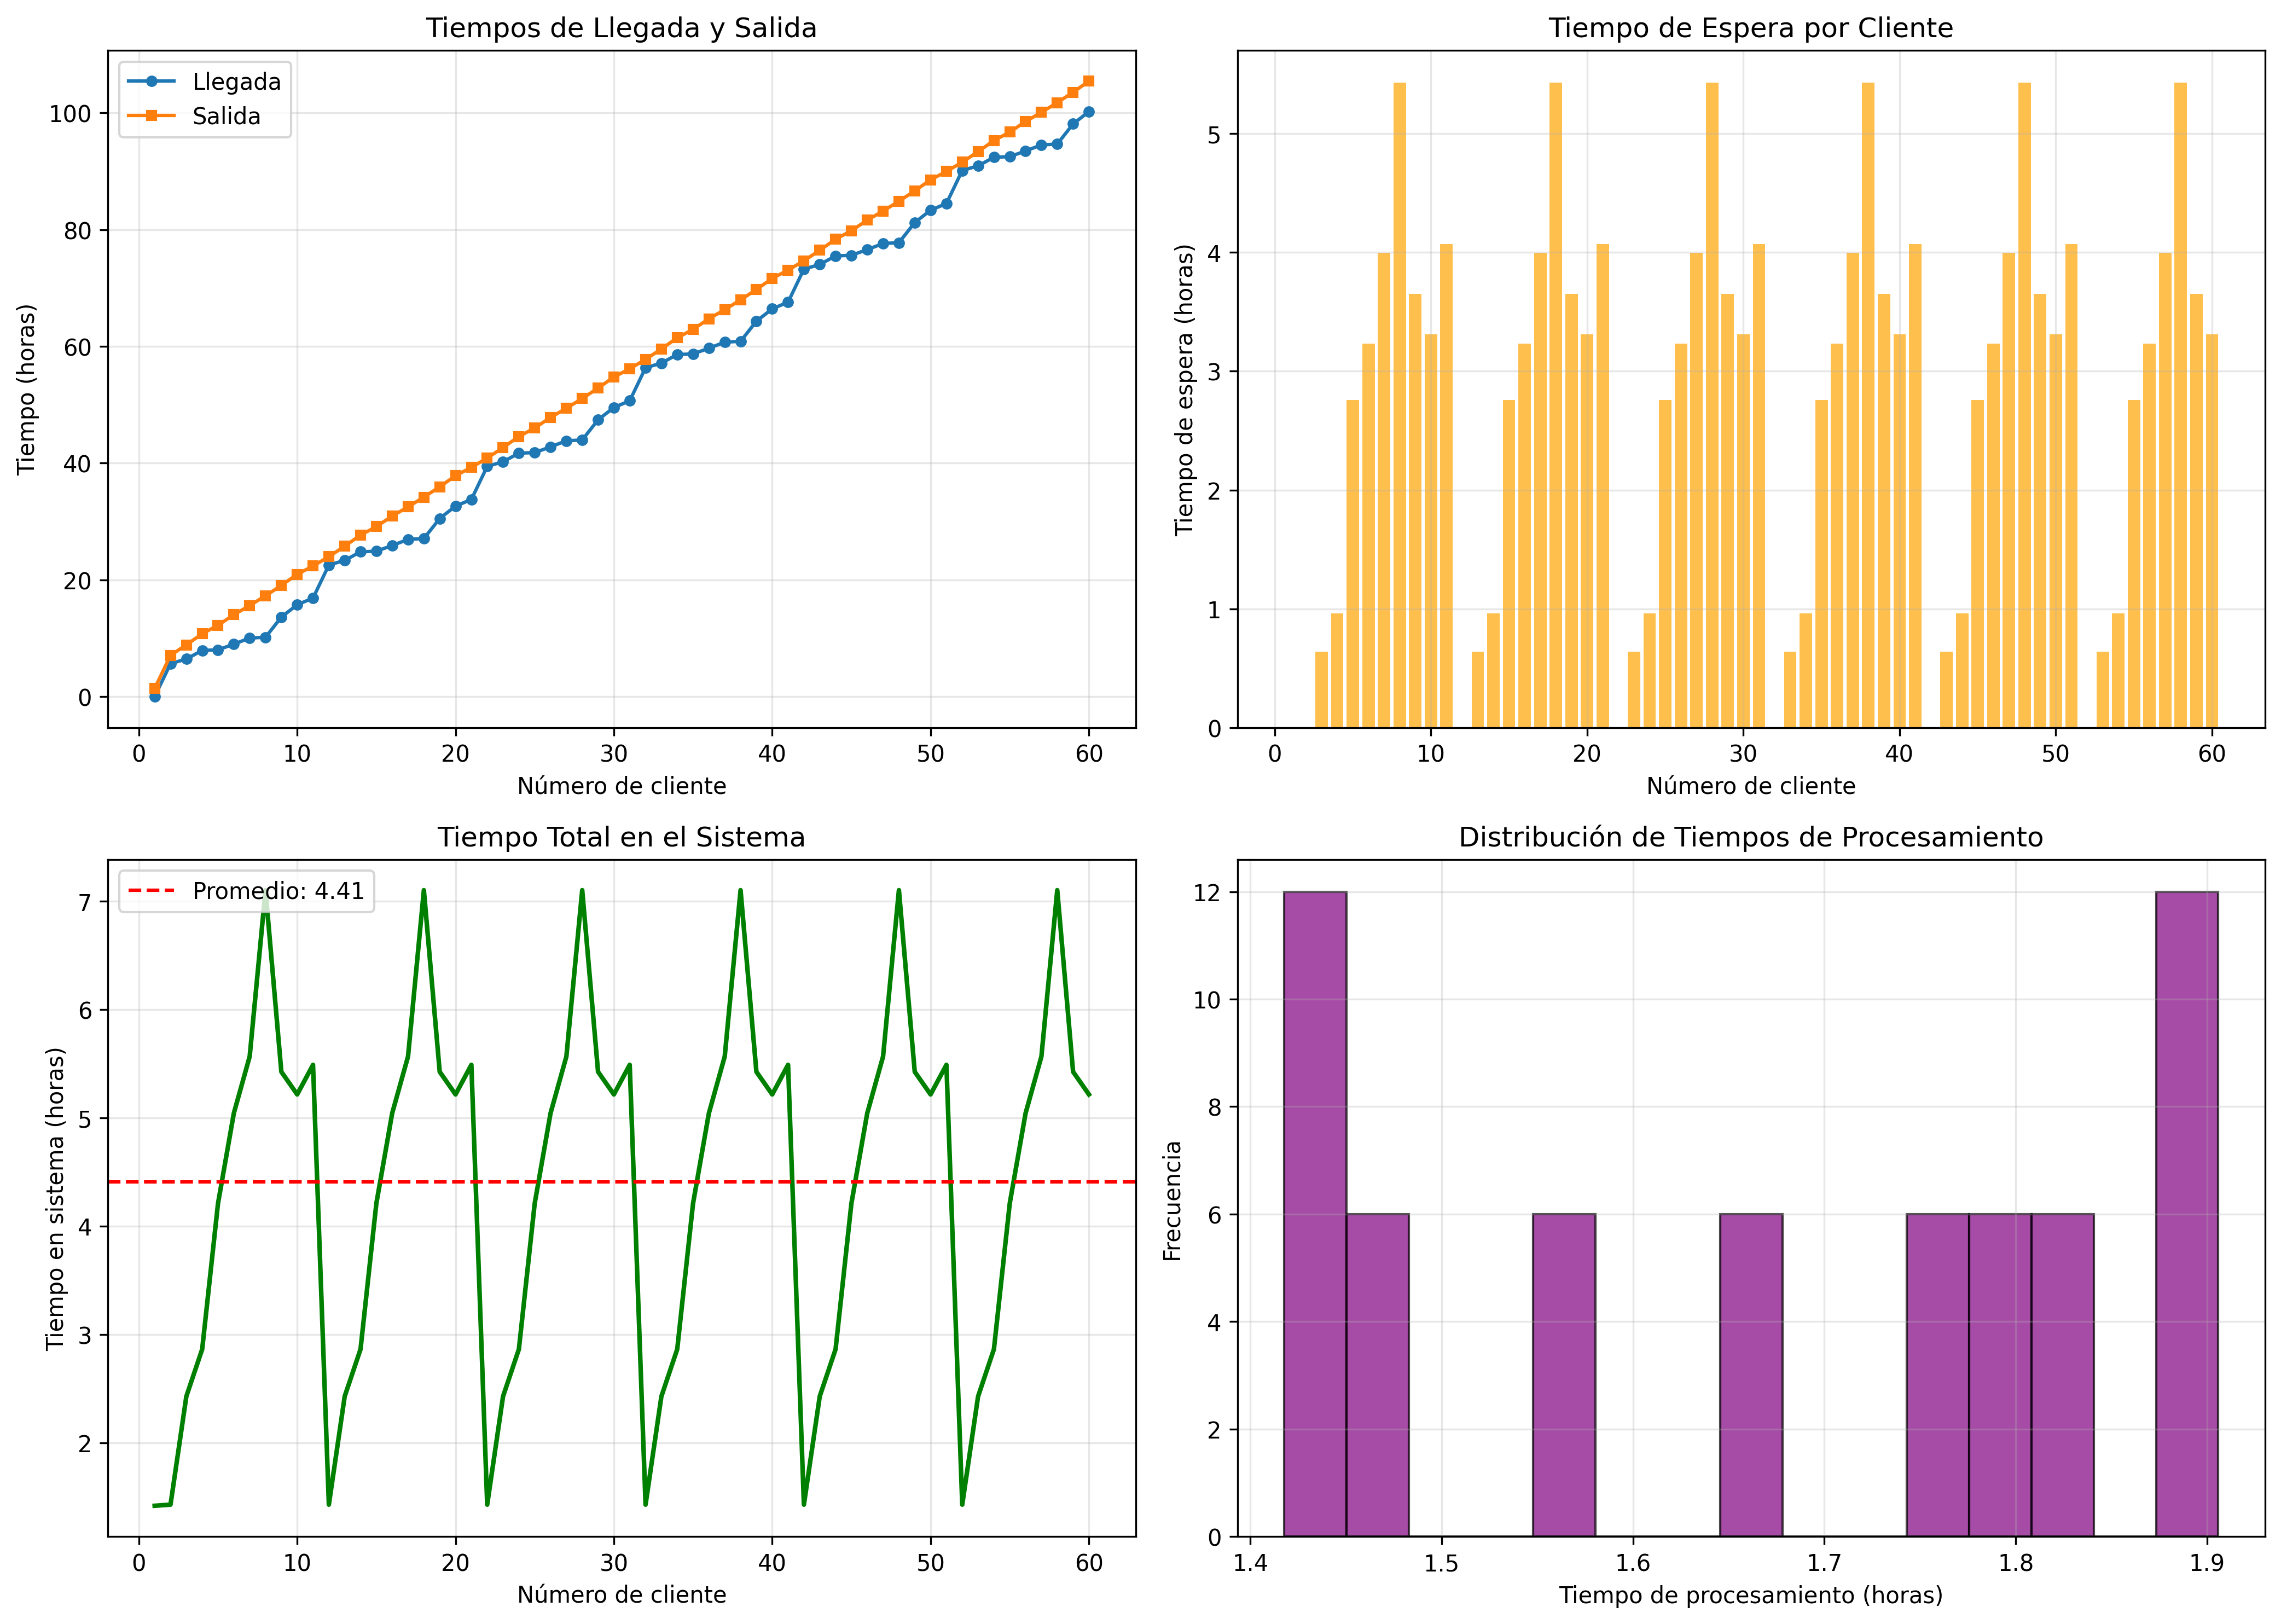
\includegraphics[width=\textwidth]{simulacion_taller.png}
\end{figure}

\end{document}
